%\documentclass[a4paper,12pt,final,twoside]{scrartcl}
\setcounter{secnumdepth}{3}
\setcounter{tocdepth}{5}

\usepackage[utf8]{inputenc}
\usepackage[T1]{fontenc}
\linespread{1.4}
\usepackage{dsfont}
\usepackage{amsfonts}
\usepackage{amsmath}
\usepackage{amssymb}
\usepackage{amsthm}
\usepackage{mathtools}
\usepackage{mathbbol}
\usepackage{amsmath1}
\usepackage[ngerman]{babel}
\usepackage{bibgerm}
\usepackage[pdftex]{graphicx}
%\usepackage{mathpazo}
\usepackage{floatflt}
%%\usepackage{epsfig}
\usepackage{wrapfig}
\usepackage{graphicx}
\usepackage{tabularx}
\usepackage{caption} 
\usepackage{multicol} 
\usepackage{mathrsfs}
%\usepackage{pspicture}
%\usepackage{eepic}
%\usepackage{epic}
%\usepackage{trfsigns}

%\usepackage[ansinew]{inputenc}
\usepackage{longtable,array,dcolumn}
%\usepackage{ngerman}
\usepackage{epic}
\usepackage{rotate}
\usepackage{graphpap}
\usepackage{amssymb}
\usepackage[squaren]{SIunits}
\usepackage{curves}
\usepackage{float}
\usepackage{array}
\usepackage{enumerate}
\usepackage{marvosym}
\usepackage{slashed}%für feynmanslsash
\usepackage[breaklinks,pdfborder={0 0 0}]{hyperref}
\usepackage{ulem}	%angeblich funktioniert dann
\let\underbar\uline	%underbar in math auch bei greek letters
\usepackage{multirow}
%\usepackage{multicolumn}
\usepackage{enumitem}


\setlength{\parskip}{12pt}
\setlength{\parindent}{0mm}
%\newcommand{\grad}{\ensuremath{^{\circ}}
%\renewcommand{\figurename}{Abb.}		% mit usepackage caption2
%\renewcommand{\captionfont}{\small \itshape}	% mit usepackage caption2
%\setkomafont{caption}{\small \itshape}		%sollte mit caption im userpackage funktionieren
%\setkomafont{captionlabel}{\small , \itshape}	%sollte mit caption im userpackage funktionieren
\captionsetup{font = {small, sf}} %mit it anstelle von sf gibts kusiv

\date{2009-20-10}
\newcommand{\kreis}[1]{
 \qbezier(-#1,0)(-#1,#1)(0,#1)
  \qbezier(0,#1)(#1,#1)(#1,0)
  \qbezier(#1,0)(#1,-#1)(0,-#1)
  \qbezier(0,-#1)(-#1,-#1)(-#1,0)}
\newcommand{\s}{\ \big| \ }
\newcommand{\lo}{\left <}
\newcommand{\ro}{\ri >}
\newcommand{\g}{&=&}

\newcommand{\ham}{\mathcal H}
\newcommand{\hil}{\mathscr H}
\newcommand{\fok}{\mathscr F}
\newcommand{\wh}{\widehat}
%\newcommand{\left}{\left}
\newcommand{\ri}{\right}
\newcommand{\Sp}{\text{Sp}}
\newcommand{\babsatz}{\par \begingroup \leftskip=2cm}
\newcommand{\eabsatz}{\par\endgroup}

\newcommand{\D}{\text{\itshape D}}
\newcommand{\Lr}{\mathcal L }%\textit{L}}
\newcommand{\rot}{\text{rot}}
\newcommand{\divergenz}{\text{div}}
\newcommand{\grad}{\text{grad}}
\newcommand{\grat}{${}^{\circ}$}
%\newcommand{\tanh}{\text{tanh}} already defined

\newcommand{\RM}[1]{\text{\MakeUppercase{\romannumeral #1}}}
\newcommand{\dell}{\partial}
\renewcommand{\div}{\operatorname{div}}
\newcommand{\I}{\dot{\text{\i\!\i}}}
\newcommand{\e}{\mathrm{e}}
\newcommand{\ket}[1]{\mid\!\!\!\,\,{#1}\rangle}
\newcommand{\bra}[1]{\langle{#1}\!\!\!\,\,\mid}
\newcommand{\braket}[2]{\langle{#1}\!\!\!\,\,\mid\!\!\!\,\,{#2}\rangle}
\newcommand{\bracket}[3]{\langle{#1}\!\!\!\,\,\mid\!\!\!\,\,{#2}\!\!\!\,\,\mid\!\!\!\,\,{#3}\rangle}
\newcommand{\1}{\mathds{1}}
\newcommand{\EW}[1]{\langle\!\!\,\,#1\!\!\,\,\rangle}
\newcommand{\arrowbox}[1]{-\!\!\!\!\:\text{(#1)}\!\!\!\;\;\!\!\!\rightarrow}

\newcommand{\ketI}[1]{\ket{#1}_{\!\!\;\text{I}}}
\newcommand{\ketII}[1]{\ket{#1}_{\!\!\;\text{II}}}
\newcommand{\ketIII}[1]{\ket{#1}_{\!\!\;\text{III}}}
\newcommand{\braI}[1]{\,\!_{\text{I}\!\!\;}\bra{#1}}
\newcommand{\braII}[1]{\,\!_{\text{II}\!\!\;}\bra{#1}}
\newcommand{\braketI}[2]{\,_{\text{I}\!\!\;}\braket{#1}{#2}_{\!\!\;\text{I}}\,}
\newcommand{\braketII}[2]{\,_{\text{II}\!\!\;}\braket{#1}{#2}_{\!\!\;\text{II}}\,}
\newcommand{\braketIII}[2]{\,_{\text{III}\!\!\;}\braket{#1}{#2}_{\!\!\;\text{III}}\,}
\newcommand{\bracketI}[3]{\,_{\text{I}\!\!\;}\bracket{#1}{#2}{#3}_{\!\!\;\text{I}}\,}
\newcommand{\bracketII}[3]{\,_{\text{II}\!\!\;}\bracket{#1}{#2}{#3}_{\!\!\;\text{II}}\,}


\newcommand{\up}{\ket{\uparrow}}
\newcommand{\updg}{\bra{\uparrow}}
\newcommand{\down}{\ket{\downarrow}}
\newcommand{\downdg}{\bra{\downarrow}}
\newcommand{\upup}{\ket{\uparrow\uparrow}}
\newcommand{\updown}{\ket{\uparrow\downarrow}}
\newcommand{\downup}{\ket{\downarrow\uparrow}}
\newcommand{\downdown}{\ket{\downarrow\downarrow}}

\newenvironment{itemize1}{\begin{itemize}[leftmargin=5mm,itemsep=-1ex,topsep=-1ex]}{\end{itemize}}

%\usepackage[left=2cm,right=2cm,top=1cm,bottom=1cm,includeheadfoot]{geometry}

\usepackage{fancyhdr}
\pagestyle{fancy}{\fancyhf{}
\fancyhead[LO,RE]{\footnotesize \rightmark}
\fancyfoot[C]{\footnotesize -$\,$\thepage$\;$-}
\renewcommand{\headrulewidth}{0.4pt}
\renewcommand{\footrulewidth}{0pt}}

\fancypagestyle{plain}{\fancyhf{}
\renewcommand{\headrulewidth}{0.4pt}
\fancyfoot[C]{\footnotesize -$\,$\thepage$\,$-}}

\usepackage{titlesec}
\titleformat{\section}[display]{\sffamily\bfseries\Huge\center}{Kapitel \thetitle:}{1ex}{}{}
\newcommand{\kapitel}[2]{$\;$\vspace{-1.5cm} \section[#1]{#2} \rule{17cm}{0.4pt}\vspace{3cm}}
\titleformat{\paragraph}[hang]{\sffamily\bfseries}{\thetitle:}{0ex}{\vspace{-0.15cm}}{\vspace{0.5cm}}

\title{ \vspace{1.5cm}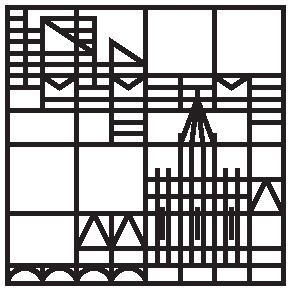
\includegraphics[width=5cm]{logo}
\\ \Large Universität Konstanz  \\ \vspace{4ex} \huge 
Skript zur Vorlesung\\ Höhere Quantentheorie und Elektrodynamik
\\ \vspace{4ex} \Large Prof. Dr. Wolfgang Belzig 
\\ Version vom 30. Juli 2012 \\ \vspace{4.5cm}
\normalsize Ursprünglichen Mitschrift von Birte Heinze im WS 09/10 \\ Ausführliche Überarbeitung von Tobias Lohse im WS 11/12 \vspace{-10cm}}
\author{}
\date{}
%\begin{document}


\subsection{Wahrscheinlichkeitsinterpretation und Messprozess}

Die Quantentheorie stellt gegenüber der klassischen Physik eine sehr Unterschiedliche Beschreibung der physikalischen Vorgänge dar. Nicht nur insofern der mathematische Formalismus sich in gravierenden Punkten von der Formulierung der klassischen Physik unterscheidet, sondern insbesondere auch, was die Bedeutung der Begriffe und die Natur der beschriebenen physikalischen Objekte angeht. 

Insbesondere die Beschreibung des Messprozess stellt dabei einen bedeutenden Unterschied zur klassischen Physik dar. Wir erinnern uns, dass bei der Messung einer Observablen der Zustand in den Eigenzustand zum zugehörigen gemessenen Eigenwert übergeht. Die Messung selbst stellt also eine Zeitentwicklung des Systems dar, welche insbesondere nicht umkehrbar ist, von der Messung abhängt und die nicht deterministische Natur der Quantenmechanik vor Augen führt. 	

Unter {\bf Determinismus} versteht man den Sachverhalt, dass der klassische Zustand, also Ort und Impuls, beliebig genau gemessen werden können. Dies ist in der Quantenmechanik nicht gegeben, da Orts und Impulsoperator keine gemeinsamen Eigenzustände haben und somit nach einer Messung von Impuls oder Ort die Information über die andere Größe verloren geht, und auch mit raffinierten Messmethoden nicht gleichzeitig exakt bestimmt werden kann. Die Zeitentwicklung in der Quantenmechanik wie in der klassischen Mechanik ist hingegen deterministisch im kausalen Sinne. Aus einem bekannten Anfangszustand lässt sich der Endzustand eines bekannten Systems, also wenn wir die Hamiltonfunktion und die Randbedingungen kennen, eindeutig ermitteln. Auch die Zeitentwicklung bei der Messung ist deterministisch, da sich der Endzustand bei bekannter Messung eindeutig ergibt. Allerdings wird beim Messprozess die nicht deterministische Natur des quantenmechanischen Zustands deutlich.  

Wir wollen uns im folgenden mit der Beschreibung des Zustands und der den Übergang zu klassischen Systemen durch sogenannte Dekohärenzen eingehen. Abschließend soll noch erörtert werden, ob die Quantenmechanik mittels verborgener Parameter erklärt werden könnte. 



\subsubsection{Messungen und Projektionspostulat}

Wir wollen noch einmal die Aussage des Projektionspostulats wiederholen: Die Messung einer durch den hermiteschen Operator $\hat{A}$ beschriebenen Observable ergibt immer einen Eigenwert $a_n$ des Operators: $\hat{A}\ket{a_n}=a_n\ket{a_n}$. Nach der Messung eines Eigenwerts $a_n$ befindet sich das System dann im zugehörigen Eigenzustand $\ket{a_n}$. Außerdem besagt die Bronsche Wahrscheinlichkeitsinterpretation, dass die Wahrscheinlichkeit das System im Zustand $\ket{a_n}$ zu finden gegeben ist durch $p_n=|\braket{a_n}{\psi}|^2$. Daraus ergibt sich dann, dass der Erwartungswert $\EW{\hat{A}}$ des Operators $\hat{A}$, also der Mittelwert der Messungen, gegeben ist durch: 
\begin{eqnarray*}
	\EW{\hat{A}} &=& \sum_n p_n\cdot a_n = \sum_n \braket{\psi}{a_n}\braket{a_n}{\psi}\cdot a_n = \bra{\psi}\underbrace{\sum_n a_n\cdot \ket{a_n}\bra{a_n}}_{=\; \hat{A}}\;\psi\rangle = \bracket{\psi}{\hat{A}}{\psi}
\end{eqnarray*}
Um die Aussagen des Projektionspostulats einfacher zu formulieren führen wir den sogenannten {\bf Projektionsoperator} $\hat{P}_a$ definieren. Ein hermetischer Projektionsoperator $\hat{P}^{\dagger}=\hat{P}$ ist dabei ganz allgemein durch die Eigenschaft gekennzeichnet, dass er den Zustand eindeutig auf seinen Eigenzustand festlegt. Es muss also gelten, dass sich das Ergebnis nach Hintereinanderausführung von Projektionen nicht ändert, dies können wir durch die Forderung $\hat{P}^2\overset!=\hat{P}$ beschreiben. 

Der Projektionsoperator $\hat{P}_a$ für den Zustand $\ket{a}$ wird dann definiert als $\hat{P}_a=\ket{a}\bra{a}$. Es ist leicht ersichtlich, dass dieser die obige Forderung erfüllt: $\hat{P}_a^2=\ket{a}\braket{a}{a}\bra{a}=\ket{a}\bra{a}=\hat{P}_a$. Es wir außerdem sofort klar, dass sich die Wahrscheinlichkeit das System im Zustand $\ket{a}$ zu finden als Erwartungswert des Projektionsoperators ergibt: $\EW{\hat{P}_{a_n}}=\braket{\psi}{a_n}\braket{a_n}{\psi}=|\braket{a_n}{\psi}|^2=p_n$. Dabei ist darauf zu achten, dass der Zustand $\ket{a}$ normiert ist, damit die obigen Relationen halten. Es lässt sich leicht zeigen, dass der Projektionsoperator nur die Eigenwerte 0 und 1 hat: 
\begin{eqnarray*}
	\hat{P} \ket{\lambda_P} = \lambda_P \ket{\lambda_P} &\quad\Leftrightarrow\quad& \hat{P}^2 \ket{\lambda_P} = \lambda_P\hat{P}\ket{\lambda_P}= \lambda_P^2 \ket{\lambda_P} \quad=\quad \hat{P}\ket{\lambda_P}=\lambda_P \ket{\lambda_P}
	\\
	&\quad\Rightarrow\quad& \hat{P}\ket{\lambda_P} \neq 0 \;\Leftrightarrow\; \lambda_P = 1 \quad\land\quad \hat{P}\ket{\lambda_P} = 1 \;\Leftrightarrow\; \lambda_P=0
\end{eqnarray*}
Es gilt außerdem, dass sich zu jedem Projektionsoperator $\hat{P}_a$ ein umgekehrter Projektionsoperator $\hat{Q}_a=\1-\hat{P}_a$ definieren lässt, bei dem die Zuordnung von Eigenwerten zu Eigenzuständen umgekehrt ist. Es lässt such leicht zeigen, dass dieser ebenfalls die Bedingung für einen Projektionsoperator erfüllt: $\hat{Q}_a^2=(\1-\hat{P}_a)^2=\1-2\hat{P}_a+\hat{P}_a^2=\1-\hat{P}_a=\hat{Q}_a$. Der Projektionsoperator und der umgekehrte Projektionsoperator erfüllen immer die Bedingung $\hat{P}_a \hat{Q}_a=\hat{Q}_a \hat{P}_a=0$. 



\subsubsection{Dichtematrix}

Um die statistische Beschreibung des Systems zu systematisieren ist es hilfreich das Konzept der sogenannten Dichtematrix einzuführen, welche gelegentlich auch als statistischer Operator oder Dichteoperator bezeichnet wird. Der Dichteoperator $\hat{\rho}$ ist dabei ein hermitescher Operator $\hat{\rho}^{\dagger}=\hat{\rho}$, welcher folgende Eigenschaften erfüllt: 
\begin{itemize1}
	\item Der Dichteoperators ist normiert: $\Sp(\hat{\rho})=1$. 
	\item Der Erwartungswert eines Operators $\hat{A}$ ist gegeben durch: $\Sp\big(\hat{\rho}\hat{A}\big)$. 
	\item Es gilt außerdem: $\Sp(\hat{\rho}^2)\leq1$. 
\end{itemize1}	
Die Spur eines beliebigen Operators $\hat{A}$ ist dabei definiert durch $\Sp(\hat{A})=\sum_n \bracket{n}{\hat{A}}{n}$, wobei die $\ket{n}$ eine beliebige Orthonormalbasis bilden. 


\paragraph{Reine und gemischte Gesamtheit}

In der Statistik unterscheidet man zwischen reinen und gemischten Gesamtheiten. Eine {\bf reine Gesamtheit} liegt vor, wenn alle für die untersuchte Statistik untersuchten Systeme in ein und demselben Zustand sind. Man spricht in diesem Fall auch davon, dass sich das System in einem reinen Zustand befindet. Um den Zustand $\ket{\psi}$ experiemtntell zu bestimmen oder verifizieren, muss man also wiederholt Messungen an einem identisch präparierten Objekten durchführen um die im Zustand enthaltene Wahrscheinlickeits-Aussage $\ket{\psi}=\sum_n c_n \ket{a_n}$ zu messen, wobei $|c_n|=p_n$ die Wahrscheinlichkeit für die Messung des Eigenwerts $a_n$ zum Eigenzustand $\ket{a_n}$ angibt. Wenn wir also insgesamt $N$ Messungen an identisch präparierten Systemen durchführen und $N_n$-mal den Eigenwert $a_n$ messen, so muss sich folgendes ergeben: 
\begin{eqnarray*}
	|c_n|^2 = p_n = \lim_{N\to\infty}\;\frac{1}{N}\cdot N_n \qquad\Rightarrow\qquad \EW{\hat{A}} = \sum_n p_n\cdot a_n = \lim_{N\to\infty}\; \frac{1}{N}\cdot\sum_n N_n\cdot a_n
\end{eqnarray*}
Für eine reine Gesamtheit können wir die Dichtematrix somit durch den Projektionsoperator $\hat{\rho}=\hat{P}_{\psi}$ in den Zustand des Systems $\ket{\psi}$ beschreiben: $\hat{\rho}=\ket{\psi}\bra{\psi}$. Damit gilt außerdem auch $\hat{\rho}^2=\hat{\rho}$ und $\Sp(\hat{\rho}^2)=1$

Eine {\bf gemischte Gesamtheit} liegt vor, wenn der Zustand des Systems nur statistisch gegeben ist, also eine statistische Verteilung von Zuständen im System vorliegt. Man spricht in diesem fall auch davon, dass sich das System in einem gemischten Zustand befindet, welcher durch das Ensemble der Zustände $\ket{\psi_i}$ gegeben ist. Die Wahrscheinlichkeit, dass sich ein beliebiges Element des Ensembles dann im Zustand $\ket{\psi_i}$ befindet ist gegeben durch $p_i$ und es muss gelten $\sum_i p_i=1$. Die Dichtematrix eines gemischten Zustandes ist dann gegeben durch $\hat{\rho}=\sum_i p_i \ket{\psi_i}\bra{\psi_i}$. Damit ergibt sich, dass $\Sp(\hat{\rho}^2)<1$ gilt. \\ 

Damit ergibt sich ein Kriterium um zu überprüfen, ob sich das System in einem reinen oder gemischten Zustand befindet: 
\begin{eqnarray*}
	\Sp(\hat{\rho}^2) = 1 \quad\Leftrightarrow\quad\text{reiner Zustand} &\qquad\qquad& \Sp(\hat{\rho}^2)<1 \quad\Leftrightarrow\quad\text{gemischter Zustand}
\end{eqnarray*}


\paragraph{Von Neumann-Gleichung}

Die Dynamik eines statistischen Systems, lässt sich nun auch direkt über die Dichtematrix beschreiben. Dazu verwenden wir die Schrödingergleichung (\ref{SGL}) für die einzelnen Zustände des Ensembles: 
\begin{eqnarray}
	\dell_t\ket{\psi_i}\;=&&\!\!\!\!\!\!\!\!\!\!\!\!-\frac{\I}{\hbar}\cdot\hat{\ham}\ket{\psi_i} \quad\land\quad \dell_t\;\bra{\psi_i}\;\;=\;\bra{\psi_i}\hat{\ham}\cdot\frac{\I}{\hbar}\nonumber
	\\\;\nonumber\\
	\Rightarrow\quad \dell_t\;\hat{\rho}(t) &=& \sum_i p_i\cdot \dell_t\ket{\psi_i}\bra{\psi_i} \;=\; \sum_i p_i\cdot\Big((\dell_t \ket{\psi_i})\bra{\psi_i}+\ket{\psi_i}(\dell_t\;\bra{\psi_i})\Big) \nonumber
	\\
	&=& -\frac{\I}{\hbar}\cdot\bigg( \hat{\ham}\sum_i p_i \ket{\psi_i}\bra{\psi_i} - \sum_i p_i \ket{\psi_i}\bra{\psi_i} \;\hat{\ham}\bigg) \quad=\quad -\frac{\I}{\hbar}\cdot \big[\hat{\ham},\hat{\rho}(t)\big]\qquad \label{vNGL}
\end{eqnarray}
Diese Gleichung wird als Von-Neumann-Gleichung bezeichnet und gilt für beliebige Hamiltonoperatoren. Es ist zu beachten, dass sie keinesfalls mit der Heisenbergschen Bewegungsgleichung (\ref{HGL}) zu verwechseln ist. Die Von-Neumann-Gleichung ist das quantenmechanische Analogon der Liouville-Gleichung der klassischen statistischen Mechanik. 

Mit Hilfe der formalen Lösung der Schrödingergleichung mit dem Zeitentwicklungsoperator $\hat{U}(t,t_0)$ lässt sich auch die formale Lösung der Von-Neumann-Gleichung beschreiben und wegen der zyklischen Vertauscbarkeit der Spur folgt dann: 
\begin{eqnarray*}
	&&\hat{\rho}(t) \;=\; \hat{U}(t,t_0)\,\hat{\rho}(t_0)\,\hat{U}^{\dagger}(t,t_0)
	\\
	&&\Rightarrow\quad \Sp\big(\hat{\rho}(t)\big)=\Sp\big(\hat{U}\,\hat{\rho}(t_0)\,\hat{U}^{\dagger}\big) = \Sp\big(\hat{U}\hat{U}^{\dagger}\hat{\rho}(t_0)\big) = \Sp\big(\hat{\rho}(t_0)\big) \quad\Rightarrow\quad \Sp\big(\hat{\rho}^2(t)\big)=\Sp\big(\hat{\rho}^2(t_0)\big)
\end{eqnarray*}
Somit bleibt die Dichtematrix normiert und ein reiner Zustand geht bei durch die Von-Neumann-Gleichung beschriebenen Zeitentwicklungen nie in einen gemischten Zustand über oder umgekehrt. 

Im Heisenberg-Bild ist die Dichtematrix Zeitunabhängig: $\hat{\rho}_H=\hat{\rho}(t_0)=:\hat{\rho}_0$. Der Erwartungswert eines Operators im Heisenbergbild $\hat{A}_H$ kann ebenso wie im Schrödinger-Bild geschrieben werden: $\EW{\hat{A}_H}=\Sp(\hat{\rho}_0\hat{A}_H)$. Somit bleiben alle Eigenschaften der Dichtematrix auch im Heisenberg-Bild erhalten. 


\paragraph{Spin-1/2-System}

für ein Spin-1/2-Teilchen, lässt sich zum Beispiel der Projektionsoperator für die Eigenzustände $\up$ und $\down$ des Drehimpulses in $z$-Richtung definieren als:
\begin{eqnarray*}
	\hat{P}_{\uparrow} = \frac12\cdot(\1+\hat{\sigma}_z) &\qquad& \hat{P}_{\downarrow} = \frac12\cdot(\1-\hat{\sigma}_z) = \1-\hat{P}_{\uparrow}
\end{eqnarray*}
Für eine allgemeine Spinrichtung $\vec{n}$ lassen sich dann die Projektionsoperatoren auf die Eigenzustände $\up_{\vec{n}}$ und $\down_{\vec{n}}$ dieser Spinrichtung definieren als: 
\begin{eqnarray*}
	\hat{P}_{\,\vec{n}\,\uparrow} &=& \frac12\cdot (\1+\vec{n}\cdot\hat{\vec{\sigma}}) \;=\; \frac12\cdot\Big(\1+\sum_i n_i\hat{\sigma}_i\Big)
	\\
	\hat{P}_{\,\vec{n}\,\downarrow} &=& \frac12\cdot (\1-\vec{n}\cdot\hat{\vec{\sigma}}) \;=\; \frac12\cdot\Big(\1-\sum_i n_i\hat{\sigma}_i\Big)
\end{eqnarray*}
Wobei die $\hat{\sigma}_i$ mit $i\in\{x,y,z\}$ die {\bf Pauli-Matrizen} sind, welche definiert sind als: 
\begin{alignat*}{3}
	\hat{\sigma}_x &\quad=\quad \up\downdg+\down\updg &\quad=\quad& \Bigg(\!\begin{array}{cc} 0 & 1 \\ 1 & 0 \end{array}\!\Bigg)
	\\
	\hat{\sigma}_y &\quad=\quad \I\cdot\big(\down\updg-\up\downdg\big) &\quad=\quad&\Bigg(\!\begin{array}{cc} 0 & -\I \\ \I & 0 \end{array}\!\Bigg)
	\\
	\hat{\sigma}_z &\quad=\quad \up\updg-\down\downdg &\quad=\quad&\Bigg(\!\begin{array}{cc} 1 & 0 \\ 0 & -1 \end{array}\!\Bigg)
\end{alignat*}
Dabei wurde für die Matrixdarstellung die Basis der Eigenzustände in $z$-Richtung $\up$ und $\down$ genutzt. Diese Darstellung wird häufig auch als {\bf Spinor-Raum} bezeichnet, in welchem die Basiszustände als $\up:=\chi_+$ und $\down:=\chi_-$ geschrieben und die Vektoren als Spinoren bezeichnet werden. In der Spinor-Basis kann man dann die Eigenzustände in $x$-, $y$- und $z$-Richtung als Vektoren mit folgender Form schreiben: 
\begin{alignat*}{7}
	\up_x &\;=\;\; \frac{1}{\sqrt{2}}\cdot(\up+\down) &\;=\;& \Bigg(\!\begin{array}{c} 1 \\ 1 \end{array}\!\Bigg) \qquad\qquad &\down_x &\;=\;\; \frac{1}{\sqrt{2}}\cdot(\up-\down) &\;=\;& \Bigg(\!\begin{array}{c} 1 \\ -1 \end{array}\!\Bigg)
	\\
	\up_x &\;=\; \frac{1}{\sqrt{2}}\cdot(\up+\I\down) &\;=\;& \Bigg(\!\begin{array}{c} 1 \\ \I \end{array}\!\Bigg) \qquad\qquad &\down_x &\;=\; \frac{1}{\sqrt{2}}\cdot(\up-\I\down) &\;=\;& \Bigg(\!\begin{array}{c} 1 \\ -\I \end{array}\!\Bigg)
	\\	
	\up_z &\;=\; \qquad\quad\up &\;=\;& \Bigg(\!\begin{array}{c} 1 \\ 0 \end{array}\!\Bigg) \qquad\qquad &\down_z &\;=\; \qquad\quad\down &\;=\;& \Bigg(\!\begin{array}{c} 0 \\ 1 \end{array}\!\Bigg)
\end{alignat*}
Die Pauli-Matrizen sind für die Beschreibung der Algebra von Systemen mit Drehsymmetrie von immenser Bedeutung und finden in der Teilchenphysik vielfach Anwendung. Wir werden im Abschnitt zur relativistischen Quantenmechanik darauf zurück kommen. Es sollen daher im folgenden noch einige wichtige Eigenschaften und Relationen aufgelistet werden: 
\begin{itemize1}
	\item Die Pauli Matrizen sind unitäre und hermitesche Operatoren: $\hat{\sigma}_i^2=\1$, welche die folgende algebraische Relation erfüllen: $-\I\cdot \hat{\sigma}_x\hat{\sigma}_y\hat{\sigma}_z=\1$. 
	\item Die Pauli-Matrizen verhalten sich bei Multiplikation wie folgt: 
	\begin{eqnarray*}
		\hat{\sigma}_i\cdot\hat{\sigma}_j &=& \delta_{ij}\cdot \1+\I\cdot \sum_k \varepsilon_{ijk}\cdot\hat{\sigma}_k 
	\end{eqnarray*}
	Damit ergibt sich ihr Kommutator beziehungsweise Antikommutator zu: 
	\begin{eqnarray*}
		\big[\hat{\sigma}_i,\hat{\sigma}_j\big]_-=2\I\cdot\sum_k\varepsilon_{ijk}\cdot\hat{\sigma}_k &\qquad& \big[\hat{\sigma}_i,\hat{\sigma}_j\big]_+=2\delta_{ij}\cdot\1
	\end{eqnarray*}
	Und es ergibt sich für die Spur folgender Zusammenhang: $\Sp(\hat{\sigma}_i\hat{\sigma}_j)=2\delta_{ij}$. 
	\item Es ist außerdem nützlich die folgenden beiden Relationen zu kennen, welche sich leicht aus der Algebra der Pauli-Matrizen herleiten lassen: 
	\begin{eqnarray*}
		\exp\big(\I\cdot(\vec{a}\cdot\hat{\vec{\sigma}}\;\!)\big) &=& \1\cdot \cos|\vec{a}|+\I\cdot (\vec{n}_{\vec{a}}\cdot \hat{\vec{\sigma}}\;\!)\cdot\sin|\vec{a}|
		\\
		(\vec{a}\cdot \hat{\vec{\sigma}}\;\!)\cdot(\vec{b}\cdot \hat{\vec{\sigma}}\;\!) &=& \1\cdot(\vec{a}\cdot\vec{b})+\I\cdot\hat{\vec{\sigma}}\cdot (\vec{a}\times\vec{b})
	\end{eqnarray*}
	Dabei ist $\vec{n}_{\vec{a}}=\vec{a}/|\vec{a}|$ der Normalenvektor in Richtung von $\vec{a}$. 
\end{itemize1}

Mit diesen Relationen lässt sich leicht zeigen, dass eine beliebige Drehung mit Winkel $\vartheta$ um die Achse $\vec{n}$ im Spinor-Raum beschrieben werden kann durch den unitären Dreh-Operator $\hat{D}_{\vec{n}}(\vartheta)=\exp(\I\cdot\vartheta/2\cdot \vec{n}\cdot\hat{\vec{\sigma}})$. Es fällt auf, dass für eine Drehung um $\vartheta=2\pi$ der Drehoperator $\hat{D}_{\vec{n}}(2\pi)=-\1$ wird. Eine Drehung um $2\pi$ ändert somit erstaunlicherweise das Vorzeichen eines Spinors und erst eine Drehung um $4\pi$ führt zur Identität $\hat{D}_{\vec{n}}(4\pi)=\1$. Diese Eigenschaft ist Grundlegend für Spinoren. 

Wir können außerdem nun die Eigenzustände für eine beliebige Drehung um die $x$-Achse auf die Achse $\vec{t}=(0,-\sin\vartheta,\cos\vartheta)$ ganz allgemein schreiben als: 
\begin{eqnarray*}
	\up_{\vec{t}(\!\vartheta\!\;\!)} \;=\; \Bigg(\!\begin{array}{c} \cos(\vartheta/2) \\ -\I\sin(\vartheta/2) \end{array}\!\Bigg) &\qquad& \down_{\vec{t}(\!\vartheta\;\!\!)} \;=\; \Bigg(\!\begin{array}{c} -\I\sin(\vartheta/2) \\ \cos(\vartheta/2) \end{array}\!\Bigg)
\end{eqnarray*}
Wir wollen nun an Hand einer Dichtematrix im Spinor-Raum die zuvor besprochenen Eigenschaften der Dichtematrix veranschaulichen. Dazu betrachten wir zunächst die Dichtematrix $\hat{\rho}_G$ eines Elektronenstrahls in dem die Spins $\uparrow$ und $\downarrow$ im Verhältnis 1:1 gemischt sind. Die Dichtematrix beschreibt somit einen gemischten Zustand: 
\begin{eqnarray*}
	\hat{\rho}_G = \frac12\big(\up\updg+\down\downdg\big) = \frac{1}{2}\cdot\Bigg(\!\begin{array}{cc} 1 & 0 \\ 0 & 1 \end{array}\!\Bigg) \quad\Rightarrow\quad \hat{\rho}_G^2 = \frac12 \cdot\hat{\rho}_G \neq \hat{\rho}_G
\end{eqnarray*}
Damit wollen wir die Dichtematrix eines reinen Zustands $\ket{\psi}=\big(\!\up+\e^{\;\I\alpha}\down\big)/\sqrt{2}$ vergleichen, welcher aus einer Superposition der beiden Spinrichtung mit einer eliebigen Phase $\alpha$ besteht. Die zugehörige Dichtematrix $\hat{\rho}_{\alpha}$ ist in diesem Fall gegeben durch: 
\begin{eqnarray*}
	\hat{\rho}_{\alpha} = \frac12\big(\up\updg+\down\downdg+\;\e^{-\I\alpha}\up\downdg+\;\e^{\;\I\alpha}\down\updg\big) = \frac{1}{2}\cdot\Bigg(\!\begin{array}{cc} 1 & \e^{-\I\alpha} \\ \e^{\;\I\alpha} & 1 \end{array}\!\Bigg)
\end{eqnarray*}
Wir sehen, dass sich die Dichtematrizen für den reinen und gemscihten Zustand dadurch unterschieden, dass im gemischten Zustand keine Außerdiagonalterme auftauchen. Da die Außerdiagonalterme somit nur auftauchen, wenn ein quantenmechanisch superponierter Zustand vorliegt, werden sie auch als Kohärenzen bezeichnet. Man kann sich leicht davon überzeugen, dass die Existenz von Außerdiagonaltermen in einer Matrix mit mehr als einem Eintrag mit der Bedingung $\Sp(\hat{\rho}^2)=1$ identisch ist. Wie wir schon erwähnt, kann durch eine unitäre Zeitentwicklung ein reiner Zustand nicht in einen gemischten Zustand übergehen, oder in anderen Worten: eine unitäre Transformation $\hat{U}$ kann in $\hat{\rho}'=\hat{U}\hat{\rho}\,\hat{U}^{\dagger}$ Außerdiagonaltherme von $\hat{\rho}$ nicht komplett verschwinden lassen. 

Die physikalische Signifikanz der Kohärenzen wird sofort ersichtlich, wenn man den Erwartungswert eines Operators $\hat{A}$ für die durch die beiden Dichtematrizen $\hat{\rho}_G$ und $\hat{\rho}_{\alpha}$ beschriebenen gemischten beziehungsweise ungemischten Zustände betrachtet: 
\begin{eqnarray*}
	\EW{\hat{A}}_G &=& \Sp(\hat{\rho}_G\hat{A}) = \frac{1}{2}\cdot\big(\bracket{\uparrow}{\hat{A}}{\uparrow}+\bracket{\downarrow}{\hat{A}}{\downarrow}\big) 
	\\
	\EW{\hat{A}}_{\alpha} &=& \Sp(\hat{\rho}_{\alpha}\hat{A}) = \frac{1}{2}\cdot\Big(\bracket{\uparrow}{\hat{A}}{\uparrow}+\bracket{\downarrow}{\hat{A}}{\downarrow} + 2\cdot\Re\big(\e^{\;\I\alpha}\bracket{\uparrow}{\hat{A}}{\downarrow}\big)\Big) = \EW{\hat{A}}_G+\Re\big(\e^{\;\I\alpha}\bracket{\uparrow}{\hat{A}}{\downarrow}\big)
\end{eqnarray*}
Für den Erwartungswert des Spins in $z$-Richtung macht dies wegen $\bracket{\uparrow}{\hat{\sigma}_z}{\downarrow}=0$ keinen Unterschied. Für den Spin in $x$-Richtung hingegen ergibt sich für den gemischten Zustand $\EW{\hat{\sigma}_x}_G=0$ für den reinen Zustand hingegen ergibt sich $\EW{\hat{\sigma}_x}_{\alpha}=\Re(\e^{\;\I\alpha})=\cos\alpha$ und für $\alpha\neq\pi/2$ unterscheiden sich die Ergebnisse somit. 

Mit Hilfe der allgemeinen Dichtematrix $\hat{\rho}=(\1+\vec{\Pi}\cdot\hat{\vec{\sigma}})$ für einen Strahl aus Spin-1/2-Teilchen lässt sich auch die Polarisationsrichtung $\vec{n}_{\vec{\Pi}}=\vec{\Pi}/|\vec{\Pi}|$ und der Polarisationsgrad $\Pi=|\vec{\Pi}|$ quantenmechanisch definieren. 


\paragraph{Dichtematrix von zusammengesetzten Systemen}

Wir haben gesagt, dass die Dichtematrix eines reinen Zustandes die Form $\hat{\rho}=\ket{n}\bra{n}$ hat. Dies gilt natürlich nur in einer speziellen Basis. Denn wir können den Zustand $\ket{n}$ ja auch in einer anderen Basis mit Vektoren $\ket{n'}$ entwickeln: $\ket{n}=\sum_{n'} c_{nn'} \ket{n'}$. In dieser Basis hat die Dichtematrix dann die folgende Form: 
\begin{eqnarray*}
	\hat{\rho} &=& \ket{n}\bra{n} \;\;=\; \sum_{n',n''} c_{nn'}\cdot c^*_{nn''} \ket{n'}\bra{n''}
\end{eqnarray*}
In dieser Basis besitzt die Dichtematrix also Außerdiagonalenelemente. Ein Beispiel dafür haben wir ja bereits im vorherigen Abschnitt gesehen. 

Wir wollen nun die Dichtematrix in einem zusammengesetzten System betrachten. Dabei sei die Basis in System I gegeben durch die Vektoren $\ketI{n}$ und in System II durch die Vektoren $\ketII{m}$. Die Dichtematrix des Zusammengesetzten Systems kann dann ganz allgemein geschrieben werden als:  
\begin{eqnarray*} 
	\hat{\rho} &=& \sum_{n,m,n',m'} \rho_{nmn'm'} \ketI{n}\ketII{m}\;\braII{m'}\braI{n'}
\end{eqnarray*} 
Um die Bedingungen $\Sp(\hat{\rho})=1$ und $\hat{\rho}=\hat{\rho}^{\dagger}$ zu erfüllen müssen dabei die Einschränkungen $\sum_{nm}\rho_{nmnm}=1$ und $\rho_{nmn'm'} = \rho^*_{n'm'nm}$ gemacht werden. Diese Bedingungen sind dabei erfüllt, wenn der reine Zustand im Produktraum gegeben ist durch $\ket{\psi}=\sum_{nm}c_{nm}\ketI{n}\ketII{m}$ und normiert ist, so dass gilt $\rho_{nmn'm'} = c_{nm}\cdot c_{n'm'}^*$, welches wie man leicht sieht die beiden Bedingungen erfüllt. 

Man kann nun in einem zusammengesetzten System die sogenannte {\bf partielle Spur} über eines der Teilsysteme definieren um die Wirkung eines allgemeinen Operators $\hat{A}$ auf nur eines der Teilsysteme zu beschreiben. Der reduzierte Operator $\hat{A}_{\text{red I}}=\Sp_{\text{II}}(\hat{A})$
ist dabei definiert als: 
\begin{eqnarray*} 
	&&\hat{A}\quad=\sum_{n,m,n',m'}a_{nmn'm'}\ketI{n}\ketII{m}\;\braII{m'}\braI{n'}
	\\
	\Rightarrow&&\hat{A}_{\text{red I}}=\Sp_{\text{II}}(\hat{A}) = \sum_m \bracketII{m}{\hat{A}}{m} = \sum_{n,n',m} a_{nmn'm} \ketI{n}\;\braI{n'}
\end{eqnarray*}
Die Wahrscheinlichkeit $p_m$ für die Messung einer Observablen im System II mit Eigenwert $m$ ist gegeben durch den Erwartungswert des Projektionsoperators $\hat{P}_m=\ketII{m}\;\braII{m}$: 
\begin{eqnarray*}
	p_m &=& \EW{\hat{P}_m}\;=\; \Sp\big(\ketII{m}\;\braII{m}\;\hat{\rho}\big) = \sum_{n'm'}\;\braI{n'}\underbrace{\braketII{m'}{m}}_{=\;\delta_{mm'}}\;\braII{m}\hat{\rho} \ketI{n'}\ketII{m'}
	\\ 
	&=& \sum_{n'}\braI{n'}\bracketII{m}{\hat{\rho}}{m}\ketI{n'} \;=\; \Sp_{\text{I}}\big(\bracketII{m}{\hat{\rho}}{m}\big) \;=\; \sum_n\rho_{nmnm} 
\end{eqnarray*}
Nach der Messung von $m$ im System II ist der Zustand des gesamten Systems zwar in System II kollabiert auf $\ketII{m}$, im System I ist der Zustand allerdings noch nicht eindeutig festgelegt. Die renormierte Dichtematrix $\hat{\rho}'(m)$ nach der Messung des Eigenwerts $m$ ist also gegeben durch: 
\begin{eqnarray*}
	\hat{\rho}'(m) &=& \frac{1}{\EW{P_m}}\cdot \ketII{m}\bracketII{m}{\hat{\rho}}{m}\braII{m} \;=\; \frac{1}{\sum\limits_n \rho_{nmnm}}\cdot\sum_{n,n'}\rho_{nmn'm}\ketI{n}\ketII{m}\;\braII{m}\braI{n'} 
\end{eqnarray*}



\subsubsection{Messprozess nach von Neumann}

Wir haben bereits festgestellt, dass eine unitäre Zeitentwicklung einen reinen Zustand nicht in einen gemischten überführen kann, also nicht die Kohärenz brechen kann. In der makroskopischen Welt treten allerdings üblicherweise keine quantenmechanischen Superpositionen auf: Gegenstände sind an einem eideutigen Ort zu finden und führen eindeutige Bewegungen aus. Was also führt zur Zerstörung der quantenmechanischen Superposition, welche auch als {\bf Dekohärenz} bezeichnet wird? Es muss sich um eine nicht unitäre Zeitentwicklung handeln und da wir ja wissen, dass die Messung eine nicht unitäre Zeitentwicklung darstellt liegt es nahe zu vermuten, dass der Übergang von der Quantenstatistik zur klassischen statistischen Mechanik durch das Projektionspostulat erklärt werden kann. Um dies besser zu verstehen, müssen wir uns vergegenwärtigen, dass jede Wechselwirkung mit der Umgebung im Endeffekt eine Messung darstellt, da bei der Wechselwirkung ja Information zwischen des Systemen ausgetauscht wird. Wir wollen also im folgenden den Messprozess an einem zusammengesetzten System untersuchen. 

Wir betrachten wieder ein zusammengesetztes System mit Teilsystemen I und II, welches sich zu Beginn im reinen Zustand $\ket{\psi}=\sum_{nm}c_{nm}\ketI{n}\ketII{m}$. Die Dichtematrix $\hat{\rho}=\ket{\psi}\bra{\psi}$ hat also die im vorigen Abschnitt beschriebene Form. Durch die Messung eines Eigenwerts $m$ am System II geht die Dichtematrix $\hat{\rho}$ des System dann über in die Dichtematrix $\hat{\rho}'$: 
\begin{eqnarray*}
	\hat{\rho} &\to& \hat{\rho}'(m) = \frac{1}{\EW{\hat{P}_m}}\cdot \hat{P}_m\,\hat{\rho}\,\hat{P}_m
\end{eqnarray*}
Wir stellen uns nun vor, dass System II ein Detektor mit Ablesezuständen $\ket{A(n)}$ ist und System I ein mikroskopisches Objekt ist. 

Zur Zeit $t=0$ befinde sich das System nun in einem eindeutigen Zustand des Detektors: $\ket{\psi(0)}=\sum_n c_n \ketI{n}\ketII{A}$. Nach einer Wechselwirkung zwischen Objekt und Detektor geht das System dann über im einen Zustand: $\ket{\psi(t)}=\sum_n c_n \ketI{n}\ketII{A(n)}$. Die Dichtematrix des Systems $\hat{\rho}(t)$ ist somit gegeben durch: 
\begin{eqnarray*}
	\hat{\rho}(t) &=& \sum_{n,n'} c_nc^*_{n'} \ketI{n}\ketII{A(n)}\;\braII{A(n')}\braI{n'}
\end{eqnarray*}
Der Detektor befindet sich somit in einem Überlagerungszustand. Dabei gehen wir davon aus, dass es sich um einen idealer Detektor handelt, bei dem verschiedene $A(n)$ unterscheidbar sind: $\braketII{A(n)}{A(n')}=\delta_{nn'}$. Wir wollen nun betrachten, was das ablesen des Detektors am Zustand des Objekts ändert: 
\begin{itemize1}
	\item Wenn wir den Detektor nicht ablesen, so befindet sich das Objekt in einem Zustand, welcher durch die reduzierte Dichtematrix $\hat{\rho}_{\text{red I}}$ beschrieben wird, welche wegen der unterscheidbarkeit der Zustände $\ketII{A(n)}$ gegeben ist durch: 
	\begin{eqnarray*} 
		\hat{\rho}_{\text{red I}} &=& \Sp_{\text{II}}\big(\hat{\rho}(t)\big) = \sum_n |c_n|^2 \ketI{n}\;\braI{n}
	\end{eqnarray*} 
	Die Kohärenzen verschwinden also, aber das System befindet sich noch in einem statistischen Gemisch der Zustände $\ketI{n}$. 
	\item Wenn wir am Detektor einen Eigenwert $A(n)$ ablesen, so kollabiert der Zustand und wird auf den reinen Zustand $\ketI{n}$ reduziert. Die Dichtematrix ist dann also durch den Projektor gegeben: $\hat{\rho}_n=\hat{P}_n=\ketI{n}\;\braI{n}$
\end{itemize1}
Wir haben somit eine Theorie gefunden, welche den Messvorgang etwas genauer beschreibt, indem es die Wechselwirkung zwischen Detektor und Objekt direkt beschreibt. Dabei mag es zunächst etwas seltsam erscheinen, dass durch die bloße Anwesenheit des Detektors die Kohärenzen wie oben erwähnt auch ganz ohne ablesen verschwinden. Dies wird etwas klarer, wenn wir bedenken, dass die Anwesenheit des Detektors ja nichts anderes als die Kopplung an ein umgebendes System bedeutet. Im allgemeinen wird dieses System immer einen Anteil haben, welcher nicht als Detektor fungiert und dessen Zustand somit auch nicht abgelesen wird, wir können diesen als ein weiteres System III beschreiben. Da im allgemeinen der Einfluss einer solchen beliebigen Umgebung $\ketIII{\!\,U(n)\,}$ aber einen distinkten Einfluss auf das Objekt haben wird, hält die Bedingung $\braketIII{U(n)}{U(n')}=\delta_{nn'}$. Da diese Umgebungsfunktion $U(n)$ nicht gemessen wird, reduziert sich die Dichtematrix des Systems also immer auf $\Sp_{\text{III}}\big(\hat{\rho}(t)\big)$ und die Kohärenzen verschwinden somit. Mit diesem Modell können wir also nun erklären, warum quantenmechanische Superpositionen bei Kopplung an eine Umgebung verschwinden. Warum treten dann aber überhaupt kohärente Zustände auf? Nun es ist zwar immer eine Umgebung vorhanden, aber die Wechselwirkung zwischen Umgebung und Objekt geschieht über eine gewisse Zeit hinweg. Die Kohärenzen verschwinden also nicht instantan, sondern werden je nach stärke der Kopplung über einen charakteristischen Zeitraum hinweg langsam kleiner. Der Zeitraum, indem das Objekt sich in einem ausreichend kohärenten Zustand befindet wird dabei als {\bf Kohärenzzeit} beschrieben. Um diese Kohärenzzeit näher zu bestimmen, bedarf es einer genaueren Theorie der Wechselwirkung zwischen Objekt und Umgebung, welche als Dekohärenztheorie bezeichnet wird und in der Quanteninformationstheorie einen wichtigen Stellenwert einnimmt. 


\paragraph{Schrödingers Katze}

Die obigen Überlegungen zum Messprozess werden allerdings trotz alledem einige gravierende Fragen zur Interpretation der Quantenmechanik auf. Besonders deutlich wird das am sogenannten Beispiel von Schrödingers Katze. Dieses verdeutlicht die (scheinbar) paradoxen Konsequenzen der Kopplung eines makroskopischen Systems an ein quantenmechanisches System. 

Wir stellen uns eine Katze vor, welche in einer Stahlkammer eingesperrt ist, zusammen mit einem Mechanismus, der ein tödliches Gift in die Stahlkammer entlässt, welches die Katze mit Sicherheit tötet. Dieser Tötungsmechanismus ist nun an die Messung des Spins eines Teilchens gekoppelt. Somit ist der Zustand der Lebendigkeit der Katze, welcher durch die Basiszustände tote Katze: $\ketI{\text{tot}}$ und lebendige Katze: $\ketI{\text{leb}}$ beschreiben wird, gekoppelt an den Spin des Teilchens, so dass gilt: 
\begin{eqnarray*}
	\ketI{\text{leb}} \;\Leftrightarrow\; \ketII{\uparrow} \qquad\land\qquad\ketI{\text{tot}} \;\Leftrightarrow\; \ketII{\downarrow}
\end{eqnarray*}
Das Teilchen ist so präpariert, dass es sich am Anfang in einem Überlagerungszustand befindet. Der Zustand des Systems ist somit gegeben durch: $\ket{\psi}=(\ketI{\text{leb}}\ketII{\uparrow}+\ketI{\text{tot}}\ketII{\downarrow})/\sqrt{2}$. Es sind nun folgende Fälle zu unterscheiden: 
\begin{itemize1}
	\item Im Ausgangszustand des Systems vor der Wechselwirkung mit der Umgebung befindet sich die Katze in einer quantenmechanischen Superposition der Lebendigkeitszustände. Die Dichtematrix des Systems ist gegeben durch: 
	\begin{eqnarray*}
		\hat{\rho} &=& \frac12 \ketII{\uparrow}\ketI{\text{leb}}\;\braI{\text{leb}}\braII{\uparrow} + \;\frac12 \ketII{\uparrow}\ketI{\text{leb}}\;\braI{\text{tot}}\braII{\downarrow} 
		\\
		&&\qquad\qquad +\;\frac12 \ketII{\downarrow}\ketI{\text{tot}}\;\braI{\text{leb}}\braII{\uparrow} + \;\frac12 \ketII{\downarrow}\ketI{\text{tot}}\;\braI{\text{tot}}\braII{\downarrow}
	\end{eqnarray*}
	Das heißt die Katze ist gleichzeitig tot und lebendig. Dabei muss man sich klar machen, dass es sich nach den Aussagen der Quantenmechanik nicht um eine reine statistische Superposition der Wahrscheinlichkeiten handelt, sondern um eine tatsächliche Superposition der physikalischen Zustände. 
	\item Wenn das System nun mit der Umgebung wechselwirkt, so verschwinden die Kohärenzen nach einer charakteristischen Dekohärenzzeit und die Dichtematrix wird zu: 
	\begin{eqnarray*} 
		\hat{\rho}' &=& \frac12 \ketII{\uparrow}\ketI{\text{leb}}\;\braI{\text{leb}}\braII{\uparrow} + \;\frac12 \ketII{\downarrow}\ketI{\text{tot}}\;\braI{\text{tot}}\braII{\downarrow}
	\end{eqnarray*}
	Die Katze befindet sich somit in einer statistischen Superposition der Zustände und ist entweder tot oder lebendig, wobei die Wahrscheinlichkeiten für die Messung eines der beiden Ereignisse jeweils 1/2 betragen. 
	\item Nach der Messung eines Spin-Eigenzustands kollabiert der Zustand in einen reinen Zustand. Nach der Messung von Spin $\downarrow$ ist die Dichtematrix dann gegeben durch: 
	\begin{eqnarray*}
		\hat{\rho}'' &=& \ketII{\downarrow}\ketI{\text{tot}}\;\braI{\text{tot}}\braII{\downarrow}
	\end{eqnarray*}
	Die Katze ist somit definitiv tot, wenn wir den Spin $\downarrow$ messen. Man kann also sagen, dass die Messung dieses Spinzustands die Katze tötet. 
\end{itemize1}
Schrödingers Katze stellt nicht notwendigerweise ein Paradoxon dar, da die Aussagen nicht widersprüchlich sind. Außerdem kann die Katze ja nicht beobachtet werden kann, wenn sie im quantenmechanischen Superpositionszustand gleichzeitig tot und lebendig ist. Somit widersprechen die Zustände auch keinen unmittelbaren Erfahrungswerten. Es ist jedoch eventuell etwas beunruhigend, dass der Zustand der Katze nicht notwendigerweise definitiv festgelegt ist und dass er nicht objektiv definiert werden kann, denn er hängt nun von der Kopplung des Systems des Beobachters mit dem der Katze zusammen. Diese Probleme sind allerdings mehr philosophischer Natur und gehören daher in den Bereich der Wissenschaftstheorie. 


%\subsubsection{Bellsche Ungleichung}
%
%Betrachten eine Quelle, die paarweise 2 Spin$\frac1 2$ Teilchen in einem Spin-Singlett-Zustand aussendet
%\begin{eqnarray*}
%\left|s\ro = \frac 1 {\sqrt 2}\left( \left|\uparrow\downarrow\ro - \left|\downarrow\uparrow\ro \ri).
%\end{eqnarray*}
%Die Teilchen fliegen in entgegengesetzten Richtungen. Sie werden von zwei Stern-Gerlach-Detektoren weit voneinander entfernt und weit weg von der Quelle gemessen. Der Detektor I misst bezüglich der Quantisierungsachse $\vec a$, während der Detektor II bezüglich der Quantisierungsachse $\vec b$ misst.\\
%Die Messwerte der Spins multipliziert mit $\frac 2 {\hbar}$ sind 1 oder -1. Die Messung bezüglich einer Achse wird als $A_{\vec a}$ bzw. $B_{\vec b}$ beschrieben.
%\begin{enumerate}
%
%\item {\bf Quantenmechanische Beschreibung}\\
%Berechnen die kombinierte Wahrscheinlichkeit $P_{\vec a\vec b}^{\left|s\ro}$ der Messung von $A_{\vec a}$ und $B_{\vec b}$, mit der Bedingung, dass sich die Teilchen vor der Messung in $\left|s\ro$ befindet.\\
%\underline{Zu zeigen:} \\Die Wahrscheinlichkeit $P_{\vec a\vec b}$ ist von der Reihenfolge unabhängig.
%
%\item{\bf Klassische Theorie mit sog. ,,versteckte Parametern''.}\\
%\underline{Annahme:} In der Quelle werden die Teilchen eins und zwei mit diesem versteckten/verborgenen Parametern $\lambda$ ausgestattet, die jedes mögliche spätere Messresultat bereits vorherbestimmen.
%\begin{alignat*}{2}
%A_{\vec a} &\longrightarrow & \text{Messergebnis an Teilchen }A \text{ entlang der Achse } \vec a\\
%B_{\vec b} &\longrightarrow & \text{Messergebnis an Teilchen }B \text{ entlang der Achse } \vec b
%\end{alignat*}
%Beide Messungen können nur Werte 1 oder -1 annehmen.\\
%$A$ ist unabhängig von $\vec b$\\
%$B$ ist unabhängig von $\vec a$\\
%$\lambda$ ist unabhängig von $\vec a$ und $\vec b$
%\begin{center} $\Longrightarrow$  \framebox{Lokalitätsannahme}\end {center}
%$\rho(\lambda)$ ist eine unbekannte Wahrscheinlichkeitsverteilung der $\lambda$s:\\
%\begin{eqnarray*}
%\boxed{\int d\lambda \rho(\lambda) = 1}
%\end{eqnarray*}
%Der klassische gemeinsame Erwartungswert für eine Messung von $A$ an I und $B$ an II ist gegeben durch
%\begin{eqnarray*}
%\underbrace{C_{\vec a\vec b}}_{\text{Korrelator}} = \int d\lambda \rho(\lambda)A_{\vec a}(\lambda)B_{\vec b}(\lambda)
%\end{eqnarray*}
%\underline{Bedingung:} \par \begingroup \leftskip=2cm
%Die Messungen werden weit weg voneinander durchgeführt, da sonst die Lokalitätsbedingung nicht erfüllt wäre.\\
%Zur Messung an I wird jeweils zufällig eine der beiden Achsen $\vec a$ und $\vec a'$ gewählt werden und zur Messung II $\vec b$ und $\vec b'$. Die Wahl findet in so kurzer Zeit statt, dass keine Kommunikation zwischen Detektor eins und Detektor zwei oder den Detektoren und der Quelle stattfinden kann.\par \endgroup
%Viele Messungen unter diesen Bedingungen ermöglichen es möglichst viele Werte von $\lambda$ ,,auszutesten''.\\
%$\Longrightarrow$ 4 Erwartungswerte: $C_{\vec a\vec b}$ ,$C_{\vec
%  a\vec b'}$ ,$C_{\vec a'\vec b}$ und $C_{\vec a'\vec b'}$.
%\begin{eqnarray*}
%\Rightarrow \boxed{-2 \leq C_{\vec a\vec b}- C_{\vec a\vec b'}+ C_{\vec a'\vec b}+C_{\vec a'\vec b'}\leq 2}
%\end{eqnarray*}
%Die oben umrahmte Ungleichung ist die {\bf Bellsche Ungleichung} in der Form von Clauser, Horne, Shimony und Holt. $\Rightarrow$ CHSH- Ungleichung
%
%\item{\bf Zur Berechnung von $C^{\left|s\ro} = C_{\vec a\vec b}^{\left|s\ro}- C_{\vec a\vec b'}^{\left|s\ro}+ C_{\vec a'\vec b}^{\left|s\ro}+C_{\vec a'\vec b'}^{\left|s\ro}$}\\
%Man kann zeigen, dass es Werte für die 4-Richtungen gibt, für die die Bellsche Ungleichung $\left|C^{\left|s\ro}\ri| \leq 2$ verletzt wird. $\Rightarrow$  Bedeutung ?
%
%\item {\bf Rechnung zu Punkt 1)}\\
%Rotation: allgemeine Rotationsmatrix $U$.
%\begin{eqnarray*}
%U = e^{-i\frac{\alpha}2 \vec n\vec \sigma} = \cos{\scriptstyle (\frac{\alpha}2)}-i\ \vec n \ \vec \sigma \sin{\scriptstyle(\frac{\alpha}2)}
%\end{eqnarray*}
%ist eine Drehung um die Achse in $\vec n$ um den Winkel $\alpha$. U ist unitär. Der Singlett Zustand $\left|s\ro$ ist Rotationsinvariant.\\
%z.B:
%\begin{eqnarray*}
%U = \frac 1 {\sqrt2} \left(\begin{array}{cc}1&1\\-1&1\end{array}\ri)
%\end{eqnarray*}
%Wir können o.B.d.A. die z-Achse als $\vec a$ -Achse wählen. $\vec b \rightarrow $x-y Ebene. $\theta$ ist der polare Winkel zwischen $\vec a$ und $\vec b$.\\
%Eine Messung von $A_{\vec a}$ an $\vec a \rightarrow$ kann 1 oder -1 mit der Wahrscheinlichkeit von jeweils $\frac 1 2$ ergeben oder falls $B_{\vec b}$ an $\vec b$ zuerst gemessen wurde$\rightarrow$ 1 oder -1 mit Wahrscheinlichkeit $\frac 1 2$.\\
%Man misst den Wert 1 $\rightarrow$ Zustand nach der Messung $\frac{\left|\uparrow \downarrow\ro}{\sqrt 2}$ oder man misst den Wert -1 $\rightarrow$ Zustand nach der Messung $-\frac{\left|\downarrow\uparrow\ro}{\sqrt 2}$.\\
%Wir rotieren den Spin des Teilchens zwei um die y-Achse mit der Rotationsmatrix 
%\begin{eqnarray*}
%U = e^{-i \frac{\theta}2 \sigma_y} = \left (\begin{array}{cc} \cos{\scriptstyle (\frac{\theta}2)}&-\sin{\scriptstyle (\frac{\theta}2)}\\ \sin{\scriptstyle (\frac{\theta}2)}&\cos{\scriptstyle (\frac{\theta}2)}\end{array}\ri).
%\end{eqnarray*}
%Wir führen die Eigenvektoren $\left|\uparrow\ro_{\vec b}$ und $\left|\downarrow\ro_{\vec b}$ bezüglich der Achse $\vec b$ ein.\\
%$\Rightarrow$ man bekommt in dem 1.Fall: $\left|\uparrow\ro \cdot \left ( -\sin{\scriptstyle (\frac{\theta}2)}\left|\uparrow\ro_{\vec b} + \cos{\scriptstyle (\frac{\theta}2)}\left|\downarrow\ro_{\vec b}\ri)$\\
%und im 2. Fall $-\left|\downarrow\ro \cdot \left ( \cos{\scriptstyle (\frac{\theta}2)}\left|\uparrow\ro_{\vec b} + \sin{\scriptstyle (\frac{\theta}2)}\left|\downarrow\ro_{\vec b}\ri)$.
%\begin{center}
%	\begin{tabular}[h!]{|c|c|c|}\hline
%		$A_{\vec a}$/$B_{\vec b}$ & 1 & -1 \\ \hline
%		1 & $\frac 1 2\sin^2{\scriptstyle (\frac{\theta}2)}$& $\frac 1 2\cos^2{\scriptstyle (\frac{\theta}2)}$ \\\hline
%		-1 & $\frac 1 2\cos^2{\scriptstyle (\frac{\theta}2)}$ & $\frac 1 2\sin^2{\scriptstyle (\frac{\theta}2)}$ \\\hline
%	\end{tabular}
%\end{center}
%\begin{alignat*}{4}
%\Rightarrow &P = \sin^2{\scriptstyle (\frac{\theta}2)}\quad&\text{ für}\quad&A_{\vec a}B_{ \vec b} = 1\\
%&P = \cos^2{\scriptstyle (\frac{\theta}2)}\quad&\text{ für}\quad&A_{\vec a}B_{ \vec b} = -1
%\end{alignat*}
%Wir messen zuerst $B_{\vec b} \Rightarrow$ das Ergebnis ist dasselbe ($\theta = 0$).\\
%\underline{Zum Beispiel:} \begin{alignat*}{3}
%&\theta = 0 &\rightarrow \vec a \uparrow\uparrow\vec b&\rightarrow \text{ man erhält } A_{\vec a}B_{\vec b} = -1\\
%&\theta = \pi &\rightarrow \vec a \uparrow\downarrow\vec b&\rightarrow \text{ man erhält } A_{\vec a}B_{\vec b} = 1\\
%&\theta = \frac{\pi}2 &\rightarrow \vec a \ \perp\vec b&\rightarrow \text{ Kombinierte W. sind gleich} = \frac 1 2\\
%\end{alignat*}
%$\Rightarrow$ Die Messergebnisse sind unkorreliert
%
%\item{\bf Rechnung zu Teil 2 siehe Übung}\\
%\item{\bf Rechnung zu Teil 3}\\
%Der Erwartungswert für $A_{\vec a}B_{\vec b}$ ist:
%\begin{eqnarray*}
%\lo s \ri| \ (\vec a \vec \sigma)(\vec b\vec \sigma) \ \left|s\ro \g \frac 1 2 \left( \lo \uparrow\downarrow\ri| - \lo\downarrow\uparrow\ri|\ri )(\vec a\vec \sigma)(\vec b\vec \sigma)\left (\lo \uparrow\downarrow\ri|- \lo \downarrow \uparrow\ri|\ri)^T\\
%\g \cdots = \frac 1 2 \left(-a_z b_z - (a_x-ia_y)(b_x+ib_y)-(a_x+i_y)(b_x-ib_y)-a_zb_z\ri)\\
%\g  -\vec a\vec b \rightarrow \lo s\s (\vec a\vec\sigma )(\vec b\vec \sigma)\s s\ro = -\cos{\scriptstyle (\theta_{\vec a} -\theta_{\vec b})}\\
%C^{\left|s\ro} \g -\cos{\scriptstyle (\theta_{\vec a} -\theta_{\vec b})} + \cos {\scriptstyle (\theta_{\vec a} -\theta_{\vec b'})} - \cos{\scriptstyle (\theta_{\vec a'} -\theta_{\vec b})}-\cos{\scriptstyle (\theta_{\vec a'} -\theta_{\vec b'})}\\
%\text{Z.B. }&{}& \theta_{\vec a}= 0,\quad \theta_{\vec b}= -\frac 3 4 \pi,\quad \theta_{\vec a'} = \frac{\pi}2, \quad\theta_{\vec b'} = \frac{-\pi}4\\
%\Rightarrow &{}& \boxed{C^{\left|s\ro} = 2 \sqrt{2} > 2}
%\end{eqnarray*}
%$\longrightarrow$ Die Quantenmechanik ist inkonsistent mit der Annahme von Lokalität und versteckte Variablen.\\
%Experimentell wurde dies 1982 von A.Aspect überprüft.
%\end{enumerate}



%\end{document}